\documentclass[11pt, oneside]{article}   	% use "amsart" instead of "article" for AMSLaTeX format
\usepackage{geometry}                		% See geometry.pdf to learn the layout options. There are lots.
\geometry{letterpaper}                   		% ... or a4paper or a5paper or ... 
%\geometry{landscape}                		% Activate for for rotated page geometry
%\usepackage[parfill]{parskip}    		% Activate to begin paragraphs with an empty line rather than an indent
\usepackage{graphicx}				% Use pdf, png, jpg, or eps� with pdflatex; use eps in DVI mode
								% TeX will automatically convert eps --> pdf in pdflatex		
\usepackage{amssymb}
\usepackage{amsmath}
\usepackage{parskip}
\usepackage{color}
\usepackage{hyperref}

\title{Sum of cosines}
%\author{The Author}
%\section{}
%\subsection*{}
\date{}							% Activate to display a given date or no date

\graphicspath{{/Users/telliott_admin/Dropbox/Tex/png/}}
% \begin{center} 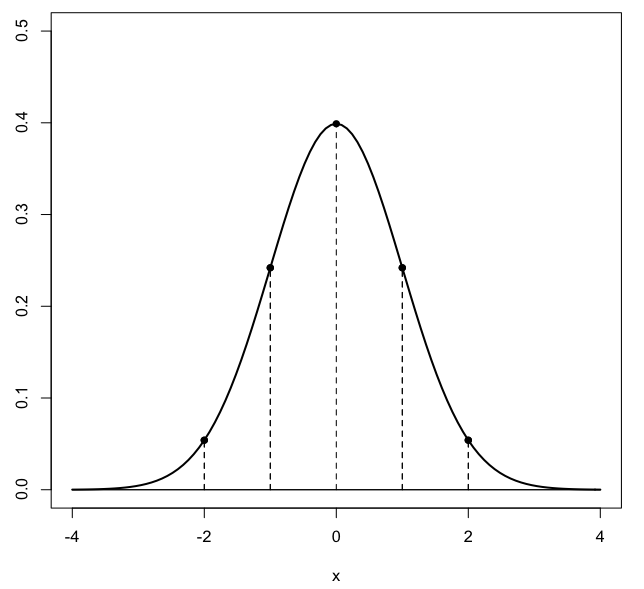
\includegraphics [scale=0.4] {gauss3.png} \end{center}
\begin{document}
\maketitle
\Large
Consider two points on the unit circle, the ray to one forms an angle $s$ with the positive $x$-axis, and similarly the other forms an angle $t$, with $s > t$.  The two points have coordinates
\[ x_1, y_1 = \cos t, \sin t \]
\[ x_2, y_2 = \cos s, \sin s \]
The square of the distance separating the two points is
\[ (x_2 - x_1)^2 + (y_2 - y_1)^2 \]
write that out
\[ (\cos s - \cos t)^2 + (\sin s - \sin t)^2 \]
\[ = \cos^2 s - 2 \cos s \cos t + \cos^2 t + \sin^2 s - 2 \sin s \sin t + \sin^2 t \]
\[ = 2 - 2 \cos s \cos t - 2 \sin s \sin t \]
Starting to look familiar?  Now, rotate the construction so the angle that was previously $t$ is equal to zero.  One of the rays now lies along the $x$-axis, and the point on the unit circle is $(1,0)$.  The angle formed by the other ray is $s - t$ and that point is $(\cos s-t, \sin s-t)$.  The square of the distance between them is
\[ (\cos s-t - 1)^2 + (\sin s-t - 0)^2 \]
\[= \cos^2 s-t - 2 \cos s-t + 1 + \sin^2 s-t \]
\[ = 2 - 2 \cos s-t \]
The distances are equal, so the squares are equal, so
\[ 2 - 2 \cos s \cos t - 2 \sin s \sin t = 2 - 2 \cos s-t \]
\[ \cos s \cos t + \sin s \sin t = \cos s-t \]
Let $-u$ = $t$
\[ \cos s \cos (-u) - \sin s \sin (-u) = \cos s+u \]
But $\cos u = \cos -u$ while $\sin -u = - \sin u$ so
\[ \cos s \cos u - \sin s \sin u = \cos s+u \]
And since $u$ and $t$ are just "dummy" variables
\[  \cos s-t = \cos s \cos t + \sin s \sin t \]
\[ \cos s+t = \cos s \cos t - \sin s \sin t  \]



\end{document}  